% !Mode:: "TeX:UTF-8"

\chapter{绪论}

\section{课题研究的背景和意义}

在软件的生命周期中,持续的代码维护是保证系统长期稳定发展的关键环节。研究表明,软件系统的维护成本在长期的项目预算中占据了60\%至80\%的比例\cite{2012Maintenance}。维护过程中,开发人员不仅要对现有代码进行修改,还要确保新增功能或修复的缺陷不会影响系统原有的稳定性和性能。为了确保软件质量,维护工作通常依赖于系统的回归测试和代码审查。具体来说,标准的代码开发流程通常包括以下三个主要步骤,如图1-1所示。

\begin{figure}[h]
\centering
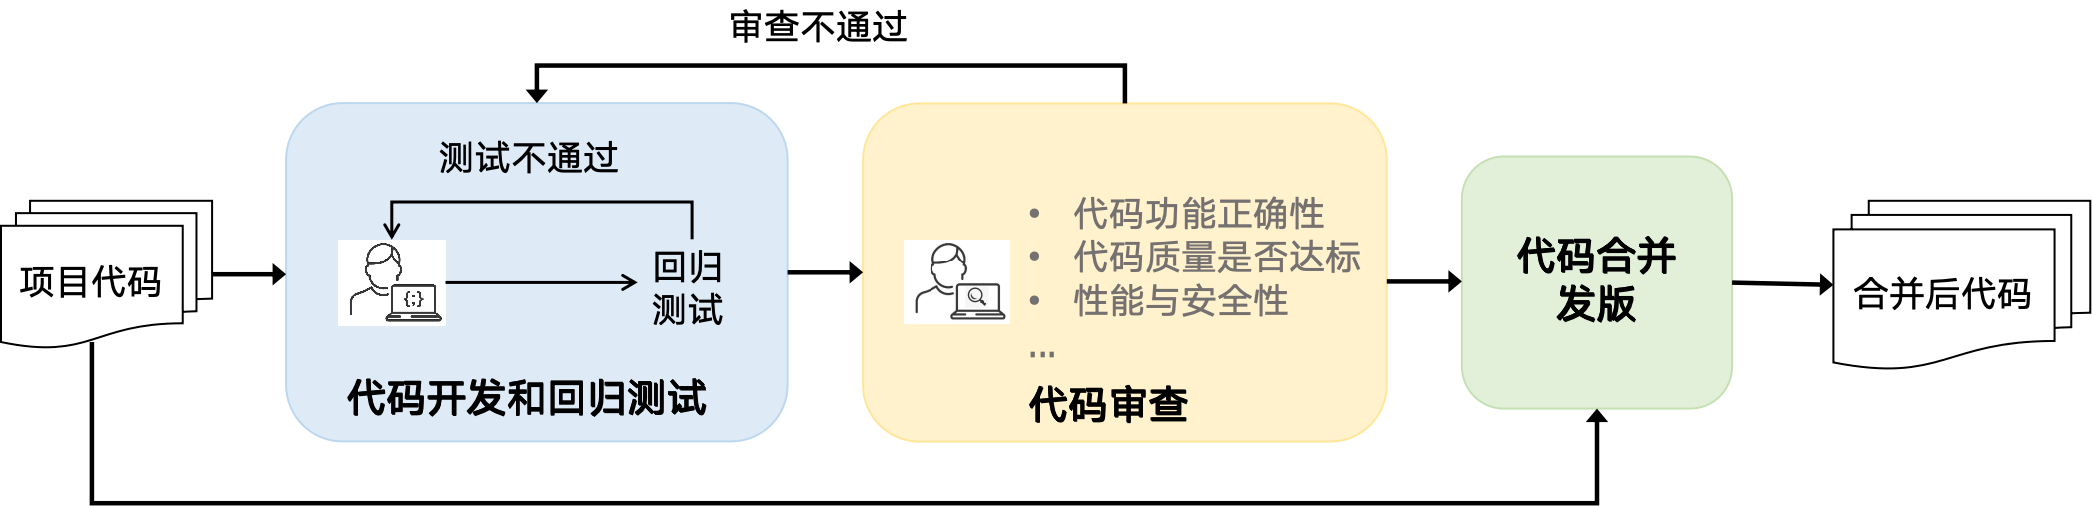
\includegraphics[width = 1.0\textwidth]{代码开发流程.png}
\caption{标准代码开发流程}
\end{figure}

(1)代码开发与回归测试:开发人员在对项目代码进行修改后,首先对修改部分进行回归测试,验证新功能是否符合需求并避免新缺陷的引入。

(2)代码审查:当测试通过后,代码将提交给审查人员进行审查。代码审查不仅仅是对代码逻辑正确性的检查,更是一个确保代码质量的重要环节。通过代码审查可以识别潜在的错误,提出代码优化建议,并统一开发团队的编码风格,从而提高代码的可维护性和可靠性。

(3)代码合并:审查通过后,修改的代码可以与原始项目进行合并,进入下一个开发周期。在此过程中,确保代码的正确性和稳定性是至关重要的,避免因合并而引入新的问题。

不论在哪一个环节,代码质量都是最重要的主题之一。而代码质量评估则是确保软件项目高效、可维护和可扩展的基础手段。随着软件系统的规模和复杂性的不断增长,代码质量直接影响到系统的稳定性、可维护性以及开发过程中的效率。尤其对于遗留系统等大型系统来讲,复杂庞大的结构和长期维护导致的系统架构腐化会让开发者在进行软件维护的时候非常困扰,常常有“牵一发而动全身”的效应,担心代码变更对系统功能的潜在不良影响。

变更影响分析(Change Impact Analysis,CIA)作为一种有效方法,能够在代码变更发生时预测变更可能带来的影响,帮助开发人员更好地理解变更对其他模块或代码的潜在影响,从而做出更加合理的设计和优化决策。因此,从代码变更影响分析的角度出发,不仅能深入理解代码变更对系统整体和各个子模块的潜在影响,还能够提高维护项目的效率\cite{2022An}。而现有的变更影响分析方法通常只关注基于静态依赖关系的影响,然而软件系统中最难以被用户察觉到,也是最容易导致功能逻辑上变更问题的是逻辑上的变更影响关系,正是因为这一关系,才导致大型系统的变更如此棘手,因此如何挖掘这类关系,分析这类关系导致的质量问题成为亟待解决的难题。

在大型软件系统中,开发者在阅读代码、掌握系统架构及模块间的关系时,常常缺乏一种与项目结构深度结合的直观展示方式。通常,开发者只能依赖于肉眼阅读代码或通过开发工具生成的类图等工具进行分析,然而这些方法所提供的信息往往是碎片化的,难以呈现系统整体的架构和模块间的依赖关系。此外,在进行代码变更时,开发者也面临着难以全面、准确地评估变更影响范围的问题,尤其是在大型系统中,单一变更可能对多个模块产生深远影响。现有的分析工具虽然能揭示代码结构或潜在问题,但难以提供系统化的、直观的质量评估。

本文从代码变更影响分析入手,提出了基于代码预训练模型和基于检索增强生成的变更影响分析方法,弥补传统方法只关注依赖型影响的不足,帮助开发者更全面、安全地进行代码维护工作。同时提出了代码审查图的软件结构和质量信息可视化方式,将分析结果结合软件代码架构直观地展示给用户,帮助开发者和审查人员更直观地理解整个项目的质量情况和代码结构,优化项目的持续维护过程,提高代码维护过程的安全性和效率。


\section{国内外研究现状及分析}

变更影响分析(Change Impact Analysis,CIA)是软件工程中用于分析代码变更对系统其他部分可能产生的影响的一种技术。研究表明,代码变更对代码质量的影响在大规模软件中尤为显著。Wenchen 等人的研究指出\cite{2013Large},在大型系统中,每个版本的补丁可能影响约 2\% 的代码,这对全面的程序回归测试提出了巨大挑战。因此,针对受变更影响的代码区域进行精确测试则是一种既高效又安全的测试方案。此方法不仅能够有效降低时间和资源成本,还能在不牺牲系统质量的前提下,减少因回归测试覆盖不足而引发的潜在漏洞或故障风险。这一策略强调了将代码变更范围与回归测试策略精细化结合的重要性,为提升软件开发和维护阶段的代码质量提供了有力支持。

自Arnold等人\cite{Arnold1996}提出变更影响分析的概念以来,它一直是代码审查的重要组成部分之一。该方法支持用户在代码变更之前对其影响进行分析,从而估计变更可能造成的负面影响,其优势可总结如下:(1)能提升代码的稳定性和可靠性。通过分析代码变更对相关模块的影响,开发者可以识别潜在的故障或不一致之处,在变更合入前发现问题,避免引入新的缺陷,从而提高系统的稳定性和可靠性。(2)有助于模块化设计和低耦合。变更影响分析能够反映出代码模块之间的依赖关系和耦合程度,通过减少不必要的耦合,增强代码的模块化特性,从而提升代码的可维护性和可扩展性。(3)有助于代码质量的提高。通过变更影响分析能够记录变更过程中的风险评估和解决措施,满足质量保证和审查的需求,提高软件开发过程的透明性和可追踪性。(4)有助于开发团队协作。变更影响分析为团队提供了清晰的变更范围和影响信息,便于团队成员之间协调工作,减少因沟通不足导致的重复工作或冲突,同时提高代码可读性,有助于开发团队更快速地理解系统,减少后期维护成本。

变更影响分析方法主要可以分为两部分,分别是静态变更影响分析方法和动态变更影响分析方法,除此之外,还有一些不专注于软件代码的方法。


\subsection{静态变更影响分析方法}

静态分析方法因其具有高覆盖率和高安全性的优势,广泛应用于对安全性要求较高的软件回归测试中。这类方法通过基于程序的中间表示(如控制流图、调用图等)来进行分析。在静态分析方法中,过程内分析方法通常依赖于程序切片、控制流和数据流等技术\cite{2004Efficient,1991Using}分析语句级别的变更影响关系,而过程间的影响分析则主要通过调用图或系统依赖图进行分析,揭示不同方法之间的依赖关系\cite{JitenderKumarChhabra2018Improved, 2011An, 2013Analyzing}。

Schrettner等人\cite{Department2013Impact}提出了一种创新的静态执行后关系(Static Execute After, SEA)方法,这是一种计算高效且足够精确的程序关系,表示代码之间的运行顺序紧密相连的情况,可以作为变更影响分析的基础。SEA的提出为程序分析提供了新的视角,其实验结果表明,通过SEA计算得到的影响关系能够发现大量的实际影响关系,显著提高了静态分析的准确性和实用性。

Sun等人\cite{5676283}提出了将变更类型与影响机制相结合的变更影响分析方法。他们认为不同类型的软件变更通常会带来不同的影响机制,因此需要根据变更的具体类型来制定相应的影响分析策略。此外,他们还指出,影响关系的精确度与初始影响关系的精确度密切相关,初始影响关系越精确,基于其计算得到的最终影响关系也会更为准确。这一发现为改进影响分析技术提供了新的思路,强调了初始数据质量对最终分析结果的重要性。

在代码变更影响的研究中,基于图的分析方法是常见的手段之一。Ufuktepe等人\cite{2021Code}针对方法间的依赖关系,利用方法调用图和影响图,提出了一种基于马尔可夫链的变更预测方法。他们通过前向切片信息计算变更后的影响概率,实验结果表明,调用图的精确率更高,而影响图则在少数情况下有更高的召回率。

Liang等人\cite{10430003}提出了一种影响集的概念,该影响集由包、类、方法、语句和变量五个层级的影响元素组合而成。通过在这五个层级上逐层搜索受影响的节点,并对这些节点进行层次化整理,最终构建出完整的层级影响结构。在此基础上,他们利用变更集定位子语句级依赖关系图中的变更节点,从多个层次分析代码变更的影响范围。

Peng等人\cite{2022An}针对传统C程序影响分析工具仅能在方法粒度上进行分析的局限性,研究了一种基于语句粒度的变更影响分析方法。该方法首先对源代码文件进行编译,提取全局信息以生成控制流图和调用图等结构。随后,将变更代码解析为不同类型变量的组合,并结合程序结构和变量变更信息进行深入的影响分析,从而更精确地评估代码变更带来的影响范围。

近年来,一些研究者尝试利用深度学习模型来研究代码变更的影响分析。Zhang等人\cite{10366673}提出了一种方法,通过构建更精细的系统依赖图并使用程序切片技术定位变更代码的影响区域,将这些区域提取为变更影响图。随后,他们采用GCN(图卷积网络)从变更影响图中提取上下文信息,并将其与抽象语法树中的语法变更数据结合起来,最终实现了对不同版本维护类型的识别。

随着软件系统复杂度的增加,单一的变更影响分析方法已经难以满足高效性和准确性的双重需求。因此,研究人员提出了混合变更影响分析技术,通过将多种CIA方法结合起来,以提高变更影响分析的准确性和健壮性\cite{2021Improving}。混合CIA技术的核心思想是将不同方法的优势互补,从而弥补单一方法的不足。研究表明,结合至少两种CIA技术的混合策略能够显著提高性能,且相比于基线技术,混合CIA方法始终表现出更好的性能改进。这一进展为变更影响分析提供了新的解决方案,尤其适用于大型复杂系统的影响分析任务。


\subsection{动态变更影响分析方法}

尽管静态影响分析在软件工程中因其较高的覆盖率和较好的安全性而被广泛应用,但其分析结果往往存在精确性不足的问题。这是因为静态分析主要依赖程序的中间表示(如控制流图、调用图等)进行推理,而这些模型无法捕捉程序在运行过程中可能出现的实际行为。为了弥补这一不足,一些研究者转向动态影响分析。与静态分析不同,动态影响分析是在程序运行时收集实际执行信息,并基于这些运行时数据计算程序中各个部分的影响关系。尽管动态分析通常能够提供更为精确的结果,但其成本较高,而且在面对复杂的系统时,无法确保分析结果的完全安全性。

尤其是在面向对象编程的系统中,由于程序实体之间的依赖关系较为复杂且难以静态建模,动态分析的结果有时会产生不精确性的影响。为了提高动态分析的精确性,Huang等人\cite{2007Precise}提出了一种专门针对面向对象程序的精确动态变更影响分析方法。该方法结合了面向对象编程的特性,能够更加准确地确定程序实体之间的实际影响关系。同时,Huang等人通过排除与变更对象无关的程序部分,显著减少了分析的规模,从而提升了分析的效率和精度。

在动态变更影响分析的精确性和可靠性方面,Cai等人\cite{2015Acom,2014Estimating}进行了深入研究。他们提出了一种实验方法,首先通过敏感性分析来评估变更影响分析的准确性,然后通过实施软件变更并观察这些变更的实际影响,进一步分析其精确度和召回率。这一方法为动态影响分析技术的有效性提供了重要的实证依据,并揭示了在实际应用中可能遇到的挑战。此外,Cai等人还提出了针对分布式系统的动态影响分析方法——DISTIA\cite{2016DistIA}。该方法通过对分布式系统中各个执行事件进行部分排序,并根据这些排序推断事件之间的因果关系,同时结合消息传递的语义预测影响在不同进程边界内外的传播情况,有效地解决了分布式系统中的影响传播问题,为分布式软件的动态影响分析提供了新的技术路径。

Wang等人\cite{王海龙0一种基于代码树分析的代码影响范围分析方法}通过词法分析器和语法分析器对源代码进行处理,将其转化为令牌和解析树,并为抽象语法树的每个节点设置预定义的权重。他们结合动态分析技术,收集代码运行时数据,并研究抽象语法树与运行时信息之间的关系,得出关联分析结果。在此基础上,构建代码影响图,并对其进行深入分析,研究代码变更如何通过影响图传播,从而得出扩散分析的结论。同时,他们追踪代码变更在抽象语法树中的传播路径,评估其可能带来的影响范围。

\subsection{其他代码变更影响分析方法}

除了上述静态和动态分析方法外,另一些研究并未直接关注软件本身,而是将关注点转向软件变更的历史库\cite{2011An, Markus2017Supporting, 2008Mining, 2014Impact, 2016Generalizing}。这些研究认为,软件变更历史记录中包含了大量与程序及其演化相关的信息,分析和挖掘这些信息能够帮助识别和预测变更对软件系统的潜在影响。这些依赖关系和变更模式可以通过数据挖掘方法、信息检索技术以及机器学习等手段进行挖掘和分析,从而为变更影响分析提供新的视角和方法。

Gethers等人\cite{2011An}采用了信息检索、动态分析和数据挖掘方法,基于历史源代码提交记录改进了变更影响方法的生成技术。通过分析过去的源代码提交,研究者能够更好地识别变更和其他程序部分之间的潜在依赖关系,从而生成更加精确的变更影响集。这一方法突出了历史数据的重要性,利用现有的变更历史信息来为未来的变更影响分析提供依据,从而提升了分析的准确性和效率。

Zanjani等人\cite{2014Impact}提出了一种结合交互历史和提交历史的方法来分析源代码变更请求。他们的创新之处在于将信息检索、机器学习和轻量级源代码分析相结合,通过构建源代码实体的语料库,来提高变更影响分析的精确度。当给定一个变更请求的文本描述时,该语料库可以被查询,并返回一个按相关性排序的最可能发生变更的源代码实体列表。这种方法能够通过历史变更请求的文本描述,准确预测哪些源代码实体可能受到影响,为开发人员提供有效的决策支持。

Rolfsnes等人\cite{2016Generalizing}致力于改进现有的耦合分析算法,尤其是在软件变更的上下文中。TARMAQ算法是他们提出的一种新型算法,在性能上明显优于ROSE\cite{2005Mining}和SVD等传统算法。TARMAQ通过挖掘代码库中的耦合关系,能够更精确地揭示源代码之间的依赖和关联,从而提高了变更影响集的生成效率和准确性。

Huang等人\cite{2021Change}则提出了一种增强型方法,通过将历史变更模式映射到当前的变更影响分析任务中,解决了跨项目场景中的变更影响分析问题。在许多实际应用中,变更影响分析不仅仅局限于单一项目,而是需要跨项目、跨系统进行分析。Huang等人的方法通过借助历史变更模式,能够在不同项目间共享和迁移影响分析的知识,进而提升了变更影响分析的普适性和适应性。


\subsection{现有方法存在的问题与分析}

静态变更影响分析方法主要通过分析软件项目各个模块的依赖关系和耦合性来提取变更影响关系。尽管该方法在某些情况下有效,但其误报率较高,导致在实际应用中可能产生较多的不准确结果。此外,动态变更影响分析方法虽然能够提供更为准确的分析结果,但其实现成本较高,且难以确保软件项目的安全性,同时由于动态运行的局限性,也存在一定程度的漏报问题。无论是静态还是动态方法,其本质上都是通过显式的模块间依赖关系来进行分析。然而,除了这些显式的依赖关系之外,仍然存在大量逻辑上的变更影响关系未被充分挖掘和揭示,这些关系往往对用户能否安全变更至关重要。

另一方面,面向变更历史的方法侧重于分析提交信息与变更代码之间的关联性,并基于这种关联性来预测新的提交可能影响的范围。这种方法分析的是自然语言与代码之间的关系,非常依赖提交信息的质量。然而,由于提交信息的质量往往难以保证,导致该方法在实际应用中可能产生较高的错误率。此外,该方法也无法应用到没有变更历史或没有提交信息的项目之上,具有一定的局限性。

现有的软件项目代码质量分析方法大多数依赖于计算度量和各种工具套件所提供的指标,这些指标虽然能够在一定程度上反映代码质量,但往往缺乏与软件项目结构的深度结合。因此,用户对软件架构的理解仍然较为抽象,缺乏直观的表现形式。



\section{本文的主要研究内容以及各章节安排}
\subsection{主要研究内容}
本文面向C/C++软件项目进行代码质量评估,旨在帮助用户在软件生命周期的各个环节全面、直观地了解软件的代码质量,了解代码各个部分的变更影响关系,帮助用户更安全地对软件代码进行维护。主要研究内容分为三个部分:代码中间表示与质量评估度量提取、面向代码质量评估的变更影响分析方法研究和代码审查图生成。

(1)代码中间表示与质量评估度量提取

代码中间表示是一种介于源代码和机器代码之间的抽象表示形式,通常用于程序分析、优化和转换等环节。通过构建合理的中间表示,可以有效地抽象出代码的结构和行为,为质量评估提供准确的依据。本文将代码转换成抽象语法树(Abstract Syntax Tree,AST),并且基于AST提取方法定义-使用链和全局变量定义-使用链,分别整理为方法摘要表和全局变量信息表。

方法摘要表和全局变量信息表为代码质量度量的计算提供了简化的、结构化的信息,使得各种质量度量的提取变得更加高效和准确。通过中间表示,代码的复杂结构和行为可以被清晰地捕捉,进而为质量度量提供更为精确的计算基础。代码质量评估度量是用于量化软件质量的各种指标。这些度量可以评估代码的模块化、可维护性、复杂度等多方面的特征。本文基于提取到的方法摘要表提取代码模块的内聚度、耦合度和复杂度相关的度量,用于评估代码的质量。

(2)面向代码质量评估的变更影响分析方法研究

本文实现了传统的静态分析方法,并设计了三种新的变更影响分析方法。基于静态分析方法根据方法摘要表和全局变量信息表计算依赖传递闭包得到变更影响关系。除此之外设计了基于克隆代码的检测方法,克隆代码指的是开发者通过复制和粘贴已有的代码片段,来创建功能类似的代码段。这种代码通常在功能上与原代码重复,因此当代码有变更的时候,这样的代码会被影响。对于有代码变更历史的软件项目,可以根据代码变更历史,通过数据挖掘的方式挖掘频繁共同更改的代码对,认为其之间存在代码变更影响关系。对于缺失代码变更历史的软件项目,将数据挖掘的到的代码对整合为数据集,训练深度学习模型,对变更影响关系进行预测。本文这四种方法结合起来,提取代码中的变更影响关系,评估其对软件质量的影响。



(3)基于代码审查图的代码架构和质量信息可视化

为帮助开发者全面了解软件项目的整体架构、模块化情况以及经过深入分析后的代码质量,本文提出了一种基于代码审查图的结果展示方式。代码审查图将整个软件项目的结构、质量度量和变更影响等信息可视化,便于开发者更直观地理解项目的各个方面,并做出相应的优化决策。

代码审查图包括多个重要组成部分:首先是代码质量度量,这涵盖了代码的复杂度、可维护性、重复性等方面的指标,能够有效反映项目的质量状况;其次是变更影响关系,该部分通过分析软件变更对其他模块和功能的影响,帮助开发者预测和规避潜在的风险;最后是模块标签,这基于软件项目的实际模块结构,通过使用大语言模型进行预测和分析,从而为开发者提供对软件模块化质量的客观评价。

在代码审查图中,节点代表项目中的关键元素,如方法和全局变量;而边则表示不同节点之间的关系,包括依赖关系、耦合关系和变更影响关系。这些边反映了不同模块或方法之间的交互和依赖,能够揭示出系统架构的潜在问题和优化点。

为了提供更加清晰的视图,代码审查图的可视化工作通过图可视化引擎G6完成,G6引擎能够高效地渲染和展示复杂的图结构,支持交互式查看和深入分析,帮助开发者快速识别问题所在。此外,所有提取和计算得到的质量评估结果还会以代码质量评估报告的形式进行详细总结,报告中将完整展示各项质量指标、分析结果和建议,确保开发者能够全面掌握软件项目的质量状态,从而进行有效的改进与优化。

\subsection{章节安排}

本文的章节安排如图1-2。

\begin{figure}[h]
\centering
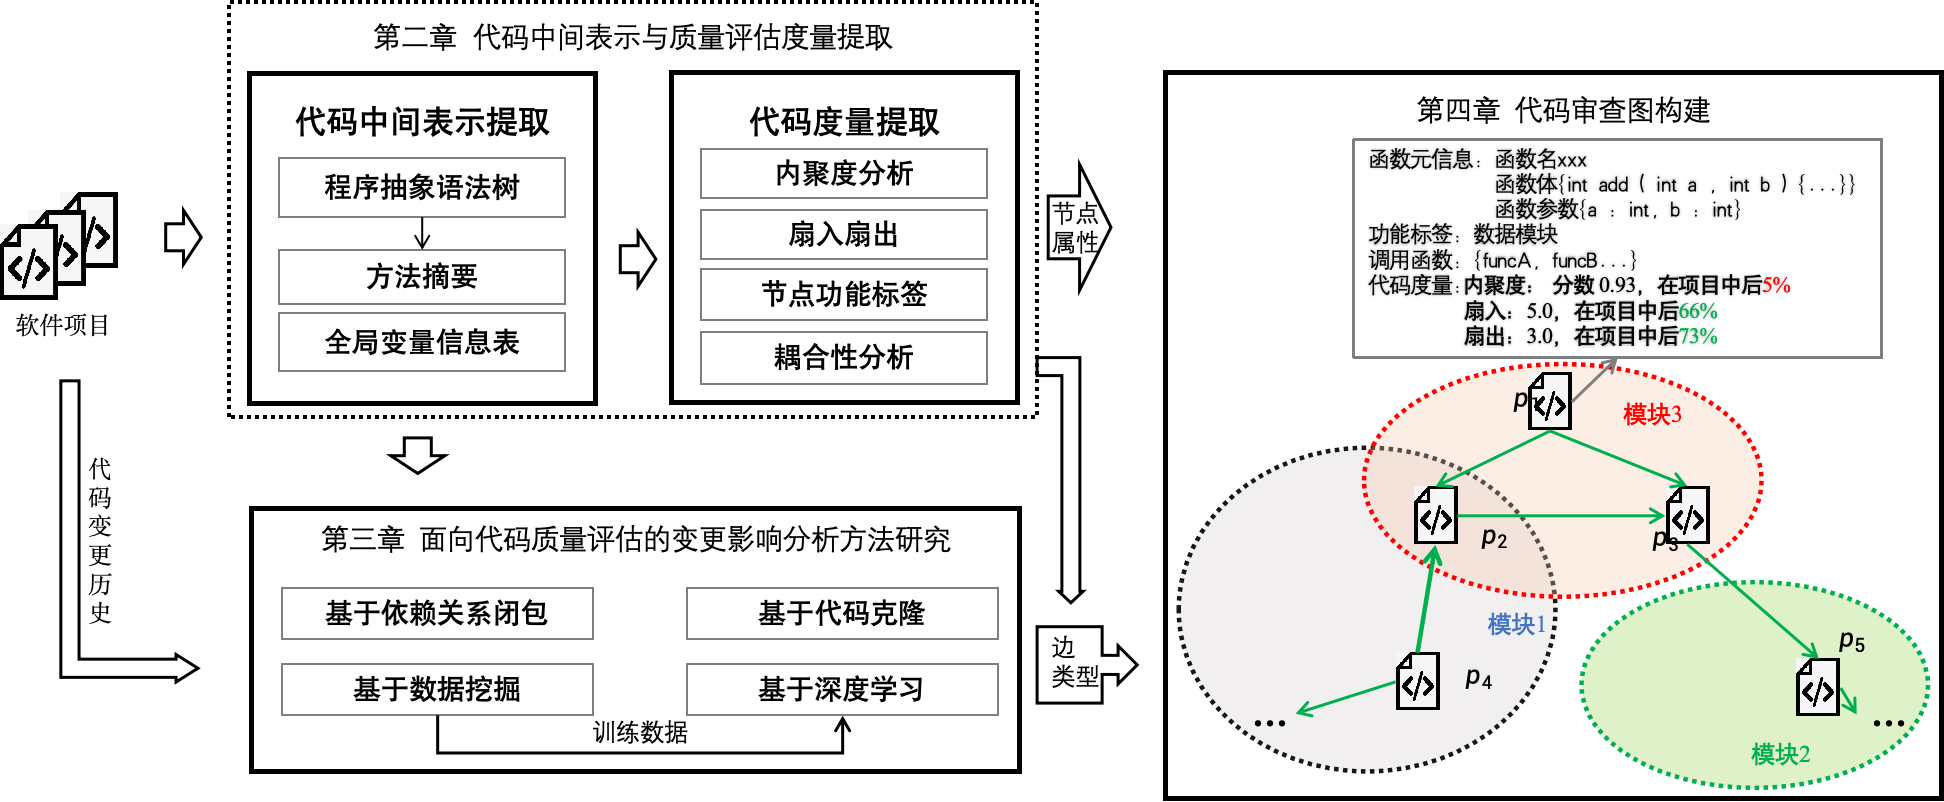
\includegraphics[width = 1.0\textwidth]{章节安排}
\caption{章节安排}
\end{figure}

第一章为绪论,首先介绍了本文的研究背景和研究现状,首先介绍了软件质量和代码变更影响的背景和意义,然后介绍了代码质量研究主题的国内外研究现状,介绍了代码质量度量套件的研究现状,并分别从静态和动态两类分析方法总结了变更影响分析的研究现状。然后介绍了本文的主要研究内容和章节安排。

第二章介绍了代码中间表示与质量评估度量提取。本章介绍了基于 clang 的抽象语法树生成方法,并且基于AST提取方法调用链和全局变量定义-使用链。基于提取的中间表示和特征,本章介绍了代码度量的提取,并进行了实验结果展示和分析。

第三章介绍了面向代码质量评估的变更影响分析方法研
究。分别介绍了基于依赖关系闭包的方法、基于代码克隆的方法、基于数据挖掘的方法和基于深度学习的方法。最后进行了实验结果展示和分析。

第四章介绍了代码审查图的生成。首先介绍了利用大语言模型生成模块标签,用于分析代码的模块化质量。其次介绍了代码审查图的构建方法,并通过图可视化引擎G6对图进行可视化,最后进行了实验结果展示和分析。



